\begin{figure}[htb!]
  \begin{center}
    \resizebox{\textwidth}{!}{
      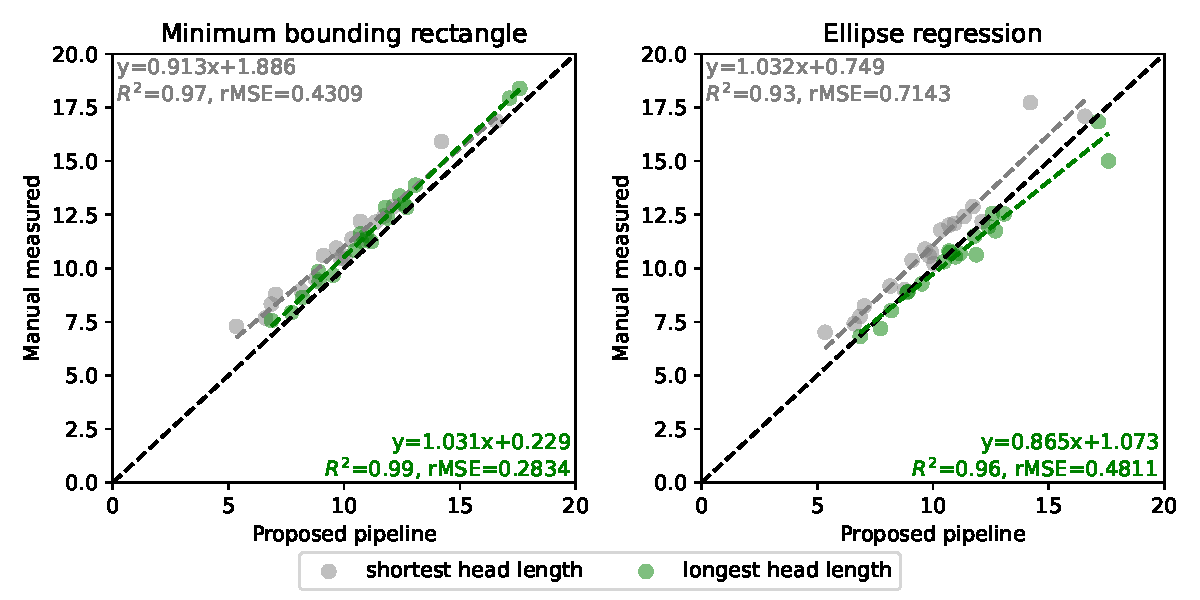
\includegraphics{figures/des/method_compare.pdf}
    }
  \end{center}
  \caption[The comparison between the proposed \replaced{close-range}{phenotyping} pipeline and manual measurement]{
    The comparison between the proposed \replaced{close-range}{phenotyping} pipeline \added{(my contribution)} and manual measurement \added{[\mbox{\citet{nishida_estimation_2023}}'s contribution]}. The shortest length and longest length of the broccoli head are compared. For the proposed pipeline, it uses two methods to estimate those lengths. One is using the length and width of the minimum bounding rectangle, the other is using the major and minor axes of the fitted ellipse.
  }
  \label{fig:des_compare}
\end{figure}